\documentclass[12pt]{article}

\usepackage{amsmath, amssymb, amsfonts}
\usepackage{geometry}
\usepackage{booktabs}
\usepackage{array}
\usepackage{multirow}
\usepackage{graphicx}
\usepackage{float}
\usepackage{indentfirst}
\usepackage{listings}
\usepackage{xcolor}

\newcommand{\x}{40pt}

\lstset{
    language=Python,
    basicstyle=\ttfamily\small,
    keywordstyle=\color{blue},
    commentstyle=\color{gray},
    stringstyle=\color{orange},
    breaklines=true,
    frame=single
}


\geometry{a4paper, margin=1in}

\title{Studies in Econometrics \\ Homework \#1}
\author{Park Jimin}
\date{2026-03-29}

\begin{document}

\maketitle

\section*{0. Setup}

Let the observed frequency matrix be $N=[n_{ij}]$, where $i=1,\dots,9$ indexes the savings-rate categories and $j=1,\dots,10$ indexes the income categories. The total sample size is
\[
n=\sum_{i=1}^{9}\sum_{j=1}^{10} n_{ij}=1021.
\]

The joint probability matrix is defined by
\[
P=[p_{ij}]=\frac{1}{n}N.
\]

The category vectors are
\[
x=
\begin{bmatrix}
0.5\\1.5\\2.5\\3.5\\4.5\\5.5\\6.7\\8.8\\12.5\\17.5
\end{bmatrix},
\qquad
y=
\begin{bmatrix}
-0.25\\-0.18\\-0.05\\0\\0.05\\0.15\\0.25\\0.40\\0.50
\end{bmatrix}.
\]

Here, income is measured in thousands of dollars per year, and the savings rate is expressed as a proportion.

\subsection*{Observed Frequency Table}

\begin{center}
\begin{tabular}{c|cccccccccc}
\toprule
Sav $\backslash$ Inc
& 0.5 & 1.5 & 2.5 & 3.5 & 4.5 & 5.5 & 6.7 & 8.8 & 12.5 & 17.5 \\
\midrule
-0.25 & 9 & 9 & 10 & 8 & 9 & 7 & 5 & 3 & 2 & 3 \\
-0.18 & 2 & 7 & 13 & 6 & 9 & 8 & 8 & 8 & 6 & 2 \\
-0.05 & 7 & 12 & 11 & 5 & 12 & 16 & 17 & 14 & 4 & 3 \\
0     & 13 & 13 & 4 & 2 & 1 & 0 & 0 & 0 & 0 & 0 \\
0.05  & 10 & 23 & 33 & 31 & 41 & 32 & 47 & 39 & 42 & 10 \\
0.15  & 2 & 9 & 9 & 12 & 16 & 20 & 42 & 54 & 24 & 21 \\
0.25  & 2 & 6 & 4 & 7 & 10 & 13 & 20 & 19 & 13 & 8 \\
0.40  & 1 & 2 & 6 & 7 & 10 & 7 & 9 & 8 & 8 & 7 \\
0.50  & 1 & 11 & 7 & 6 & 4 & 5 & 8 & 9 & 14 & 4 \\
\bottomrule
\end{tabular}
\end{center}


\subsection*{Joint Probability Table}

\begin{center}
\footnotesize{
\begin{tabular}{c|cccccccccc}
\toprule
Sav $\backslash$ Inc
& 0.5 & 1.5 & 2.5 & 3.5 & 4.5 & 5.5 & 6.7 & 8.8 & 12.5 & 17.5 \\
\midrule
-0.25 & 0.0088 & 0.0088 & 0.0098 & 0.0078 & 0.0088 & 0.0069 & 0.0049 & 0.0029 & 0.0020 & 0.0029 \\
-0.18 & 0.0020 & 0.0069 & 0.0127 & 0.0059 & 0.0088 & 0.0078 & 0.0078 & 0.0078 & 0.0059 & 0.0020 \\
-0.05 & 0.0069 & 0.0118 & 0.0108 & 0.0049 & 0.0118 & 0.0157 & 0.0167 & 0.0137 & 0.0039 & 0.0029 \\
0     & 0.0127 & 0.0127 & 0.0039 & 0.0020 & 0.0010 & 0 & 0 & 0 & 0 & 0 \\
0.05  & 0.0098 & 0.0225 & 0.0323 & 0.0304 & 0.0402 & 0.0313 & 0.0460 & 0.0382 & 0.0411 & 0.0098 \\
0.15  & 0.0020 & 0.0088 & 0.0088 & 0.0118 & 0.0157 & 0.0196 & 0.0411 & 0.0529 & 0.0235 & 0.0206 \\
0.25  & 0.0020 & 0.0059 & 0.0039 & 0.0069 & 0.0098 & 0.0127 & 0.0196 & 0.0186 & 0.0127 & 0.0078 \\
0.40  & 0.0010 & 0.0020 & 0.0059 & 0.0069 & 0.0098 & 0.0069 & 0.0088 & 0.0078 & 0.0078 & 0.0069 \\
0.50  & 0.0010 & 0.0108 & 0.0069 & 0.0059 & 0.0039 & 0.0049 & 0.0078 & 0.0088 & 0.0137 & 0.0039 \\
\bottomrule
\end{tabular}
}
\end{center}


\vspace{\x}
\section*{1. Marginal Frequencies of Income and Savings Rate}

\subsection*{Formula}

The marginal frequency vector of income is obtained by summing each column:
\[
f_X=N^\top \mathbf{1}_9,
\qquad
p_X=P^\top \mathbf{1}_9,
\]
where $\mathbf{1}_9$ is a $9\times 1$ vector of ones.

The marginal frequency vector of savings rate is obtained by summing each row:
\[
f_Y=N\mathbf{1}_{10},
\qquad
p_Y=P\mathbf{1}_{10},
\]
where $\mathbf{1}_{10}$ is a $10\times 1$ vector of ones.

\subsection*{Results}

\footnotesize{
\begin{center}
\begin{tabular}{c|cccccccccc}
\toprule
Income & 0.5 & 1.5 & 2.5 & 3.5 & 4.5 & 5.5 & 6.7 & 8.8 & 12.5 & 17.5 \\
\midrule
Frequency & 47 & 92 & 97 & 84 & 112 & 108 & 156 & 154 & 113 & 58 \\
Probability & 0.0460 & 0.0901 & 0.0950 & 0.0823 & 0.1097 & 0.1058 & 0.1528 & 0.1508 & 0.1107 & 0.0568 \\
\bottomrule
\end{tabular}
\end{center}
}

\small{
\begin{center}
\begin{tabular}{c|ccccccccc}
\toprule
Savings & -0.25 & -0.18 & -0.05 & 0 & 0.05 & 0.15 & 0.25 & 0.40 & 0.50 \\
\midrule
Frequency & 65 & 69 & 101 & 33 & 308 & 209 & 102 & 65 & 69 \\
Probability & 0.0637 & 0.0676 & 0.0989 & 0.0323 & 0.3017 & 0.2047 & 0.0999 & 0.0637 & 0.0676 \\
\bottomrule
\end{tabular}
\end{center}
}


\subsection*{Interpretation}

Looking at the marginal frequencies, the income distribution is most concentrated in the 6.7 and 8.8 categories, where the number of households is 156 and 154, respectively. By contrast, the lowest income category, 0.5, contains only 47 households, and the highest category, 17.5, contains 58 households. This suggests that the sample is centered more in the middle and upper-middle part of the income distribution rather than at the extremes.

A similar pattern appears in the savings-rate distribution. The most common savings category is 0.05, with 308 households, followed by 0.15, with 209 households. Negative savings categories such as $-0.25$ and $-0.18$ contain 65 and 69 households, respectively, so they are present in the sample but much less common than small positive savings. Taken together, the marginal frequencies suggest that most households in this sample have moderate income levels and tend to save a small but positive share of their income.




\vspace{\x}
\section*{2. Conditional Frequencies of Income Given Savings}

\subsection*{Formula}

For a given savings category $Y=y_i$, the conditional frequency of income is
\[
P(X=x_j\mid Y=y_i)=\frac{n_{ij}}{\sum_{j=1}^{10} n_{ij}}.
\]

In matrix form,
\[
P_{X\mid Y}=D_Y^{-1}N,
\]
where
\[
D_Y=\operatorname{diag}(f_Y).
\]

\subsection*{Results}

\[
P_{X\mid Y}=
\begin{bmatrix}
0.1385&0.1385&0.1538&0.1231&0.1385&0.1077&0.0769&0.0462&0.0308&0.0462\\
0.0290&0.1014&0.1884&0.0870&0.1304&0.1159&0.1159&0.1159&0.0870&0.0290\\
0.0693&0.1188&0.1089&0.0495&0.1188&0.1584&0.1683&0.1386&0.0396&0.0297\\
0.3939&0.3939&0.1212&0.0606&0.0303&0&0&0&0&0\\
0.0325&0.0747&0.1071&0.1006&0.1331&0.1039&0.1526&0.1266&0.1364&0.0325\\
0.0096&0.0431&0.0431&0.0574&0.0766&0.0957&0.2010&0.2584&0.1148&0.1005\\
0.0196&0.0588&0.0392&0.0686&0.0980&0.1275&0.1961&0.1863&0.1275&0.0784\\
0.0154&0.0308&0.0923&0.1077&0.1538&0.1077&0.1385&0.1231&0.1231&0.1077\\
0.0145&0.1594&0.1014&0.0870&0.0580&0.0725&0.1159&0.1304&0.2029&0.0580
\end{bmatrix}
\]


\begin{figure}[H]
\centering
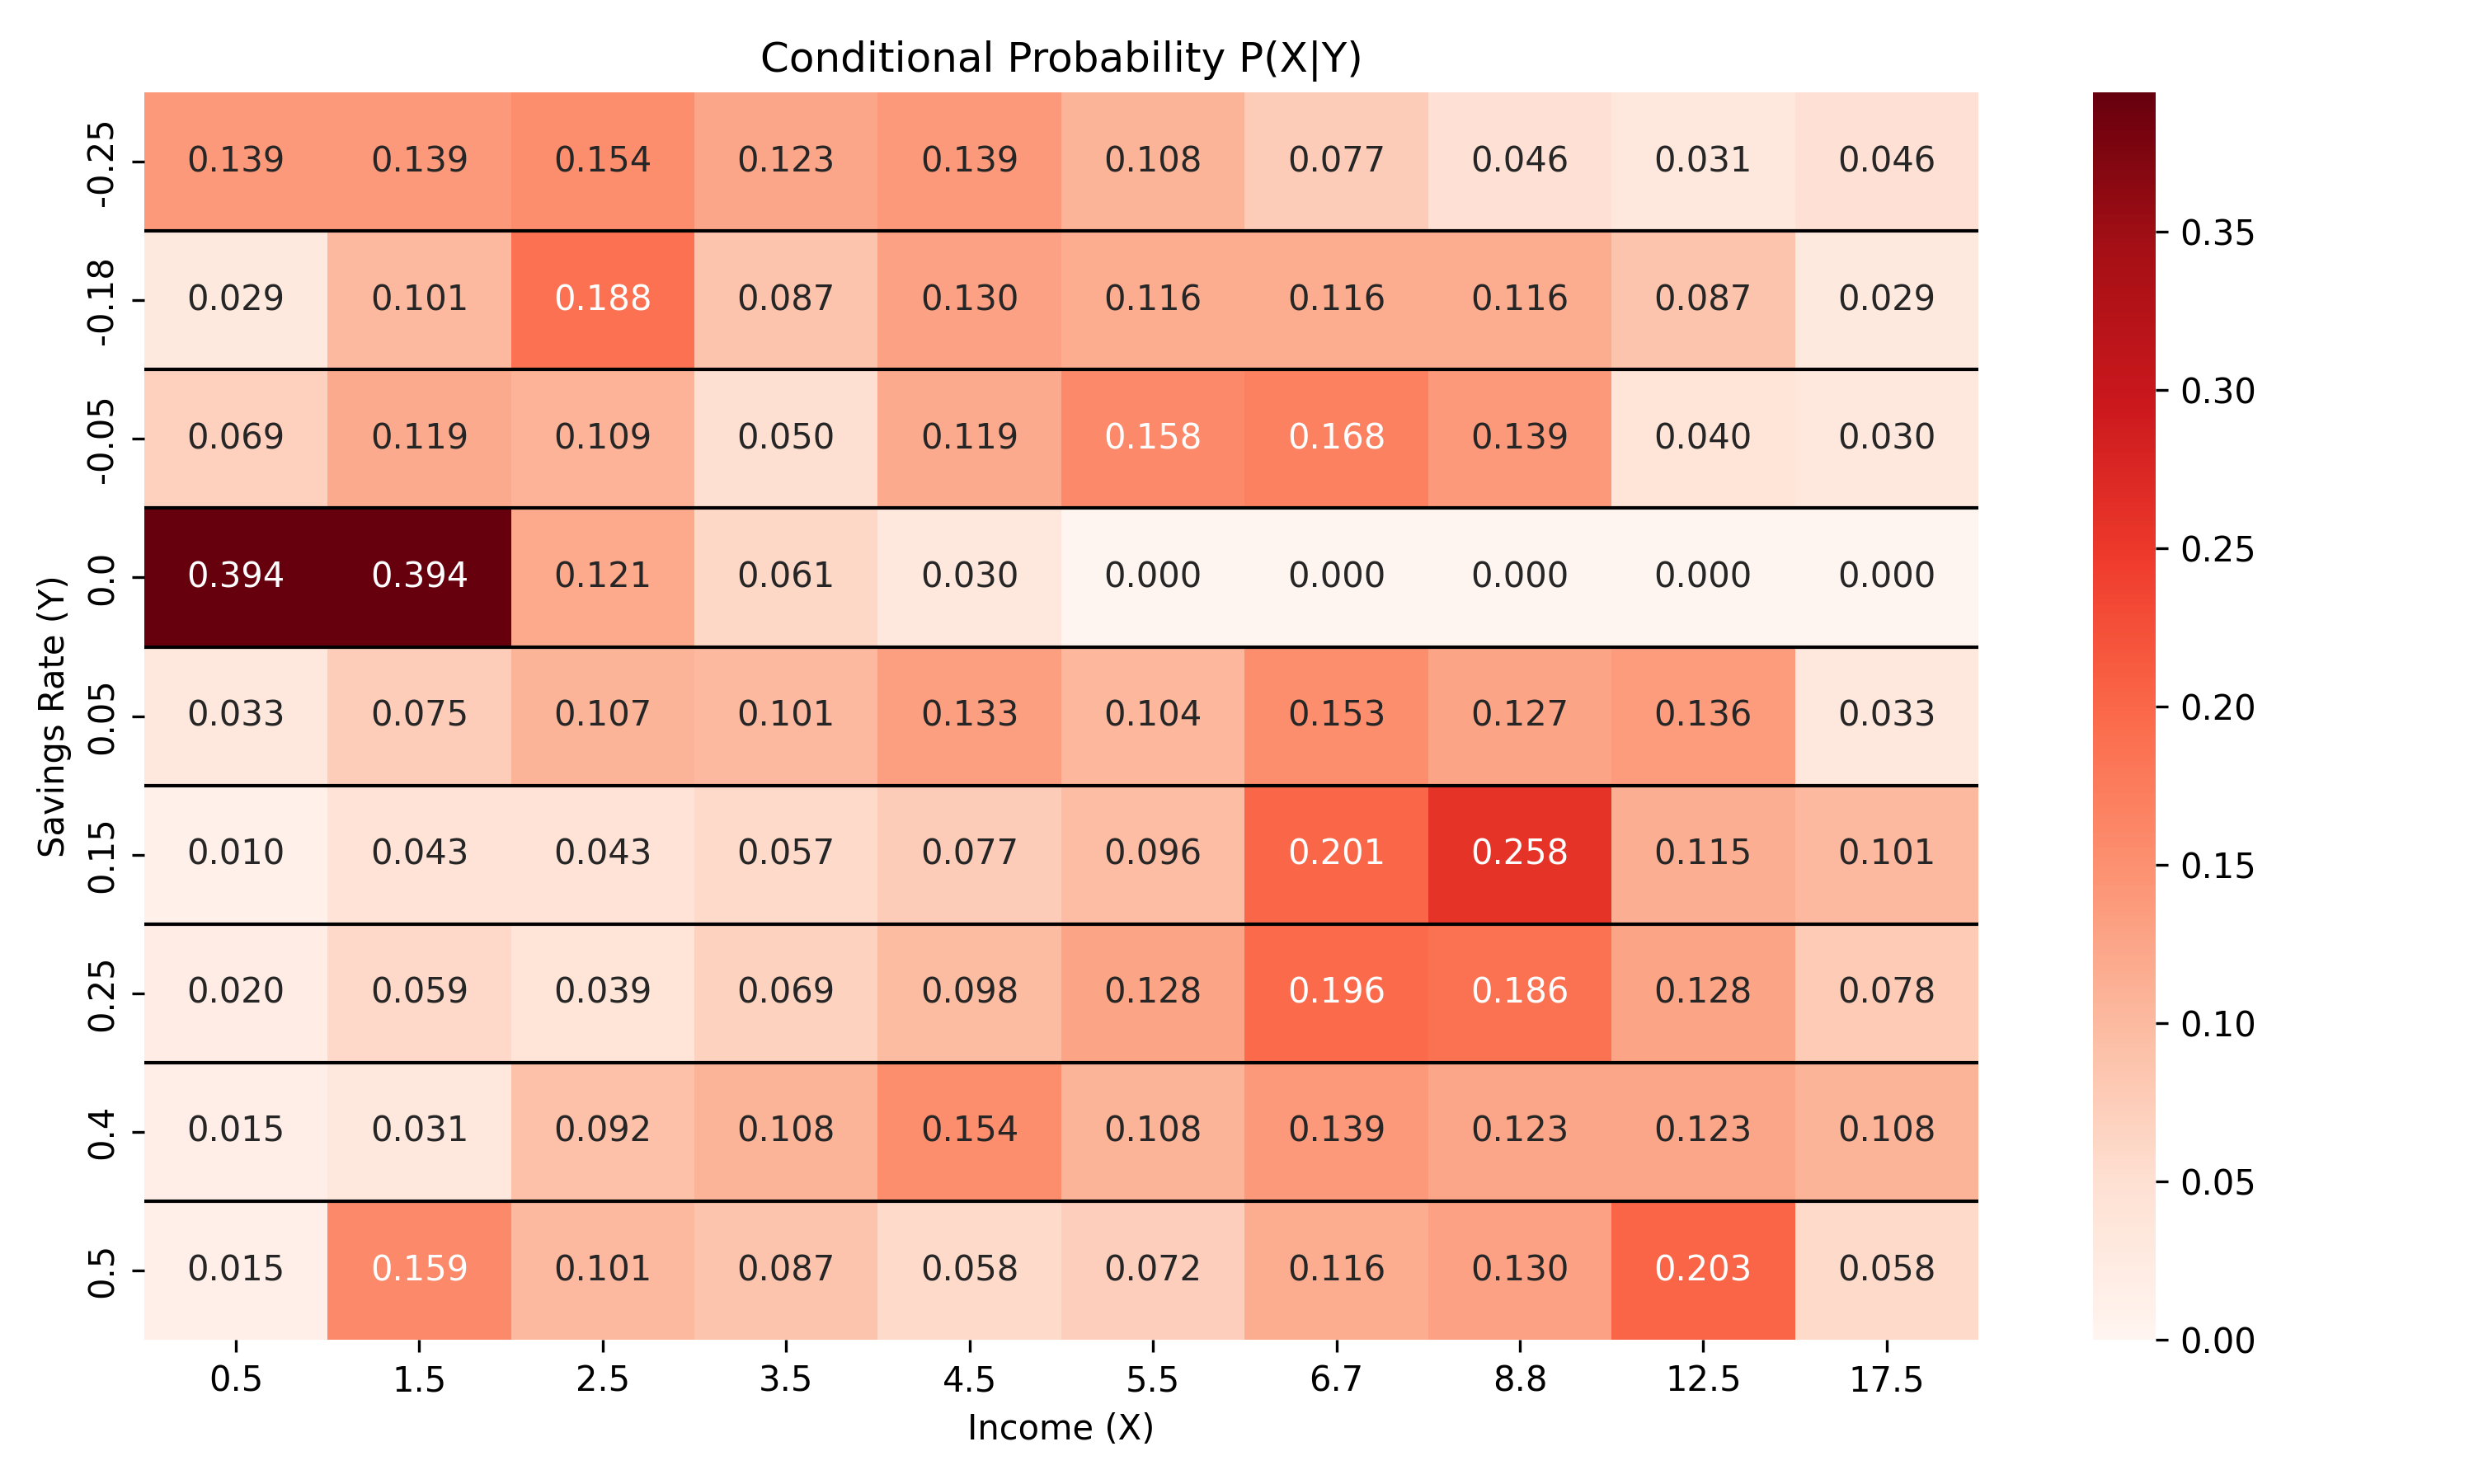
\includegraphics[width=\textwidth]{heatmap_P_X_given_Y.png}
\caption{Conditional probability $P(X|Y)$}
\end{figure}


\subsection*{Interpretation}

Each row of $P_{X\mid Y}$ shows how income is distributed within a fixed savings-rate category. For example, when the savings rate is 0, the largest conditional probabilities are attached to the two lowest income categories: both 0.5 and 1.5 have probability 0.3939. In other words, among households with zero savings, nearly 79\% are concentrated in those two lowest income groups. This makes it clear that zero savings is strongly associated with low income in this sample.

As savings rates become more positive, the distribution shifts toward higher income categories. For instance, when the savings rate is 0.15, the largest probabilities occur at income 8.8 and 6.7, with values 0.2584 and 0.2010, respectively. Likewise, when the savings rate is 0.25, the highest probabilities are again concentrated at 6.7 and 8.8, with values 0.1961 and 0.1863. Overall, the table suggests a clear tendency for higher savings rates to be associated with higher income levels.



\vspace{\x}
\section*{3. Conditional Frequencies of Savings Given Income}

\subsection*{Formula}

For a given income category $X=x_j$, the conditional frequency of savings rate is
\[
P(Y=y_i\mid X=x_j)=\frac{n_{ij}}{\sum_{i=1}^{9} n_{ij}}.
\]

In matrix form,
\[
P_{Y\mid X}=ND_X^{-1},
\]
where
\[
D_X=\operatorname{diag}(f_X).
\]

\subsection*{Results}

\[
P_{Y\mid X}=
\begin{bmatrix}
0.1915&0.0978&0.1031&0.0952&0.0804&0.0648&0.0321&0.0195&0.0177&0.0517\\
0.0426&0.0761&0.1340&0.0714&0.0804&0.0741&0.0513&0.0519&0.0531&0.0345\\
0.1489&0.1304&0.1134&0.0595&0.1071&0.1481&0.1090&0.0909&0.0354&0.0517\\
0.2766&0.1413&0.0412&0.0238&0.0089&0&0&0&0&0\\
0.2128&0.2500&0.3402&0.3690&0.3661&0.2963&0.3013&0.2532&0.3717&0.1724\\
0.0426&0.0978&0.0928&0.1429&0.1429&0.1852&0.2692&0.3506&0.2124&0.3621\\
0.0426&0.0652&0.0412&0.0833&0.0893&0.1204&0.1282&0.1234&0.1150&0.1379\\
0.0213&0.0217&0.0619&0.0833&0.0893&0.0648&0.0577&0.0519&0.0708&0.1207\\
0.0213&0.1196&0.0722&0.0714&0.0357&0.0463&0.0513&0.0584&0.1239&0.0690
\end{bmatrix}
\]


\begin{figure}[H]
\centering
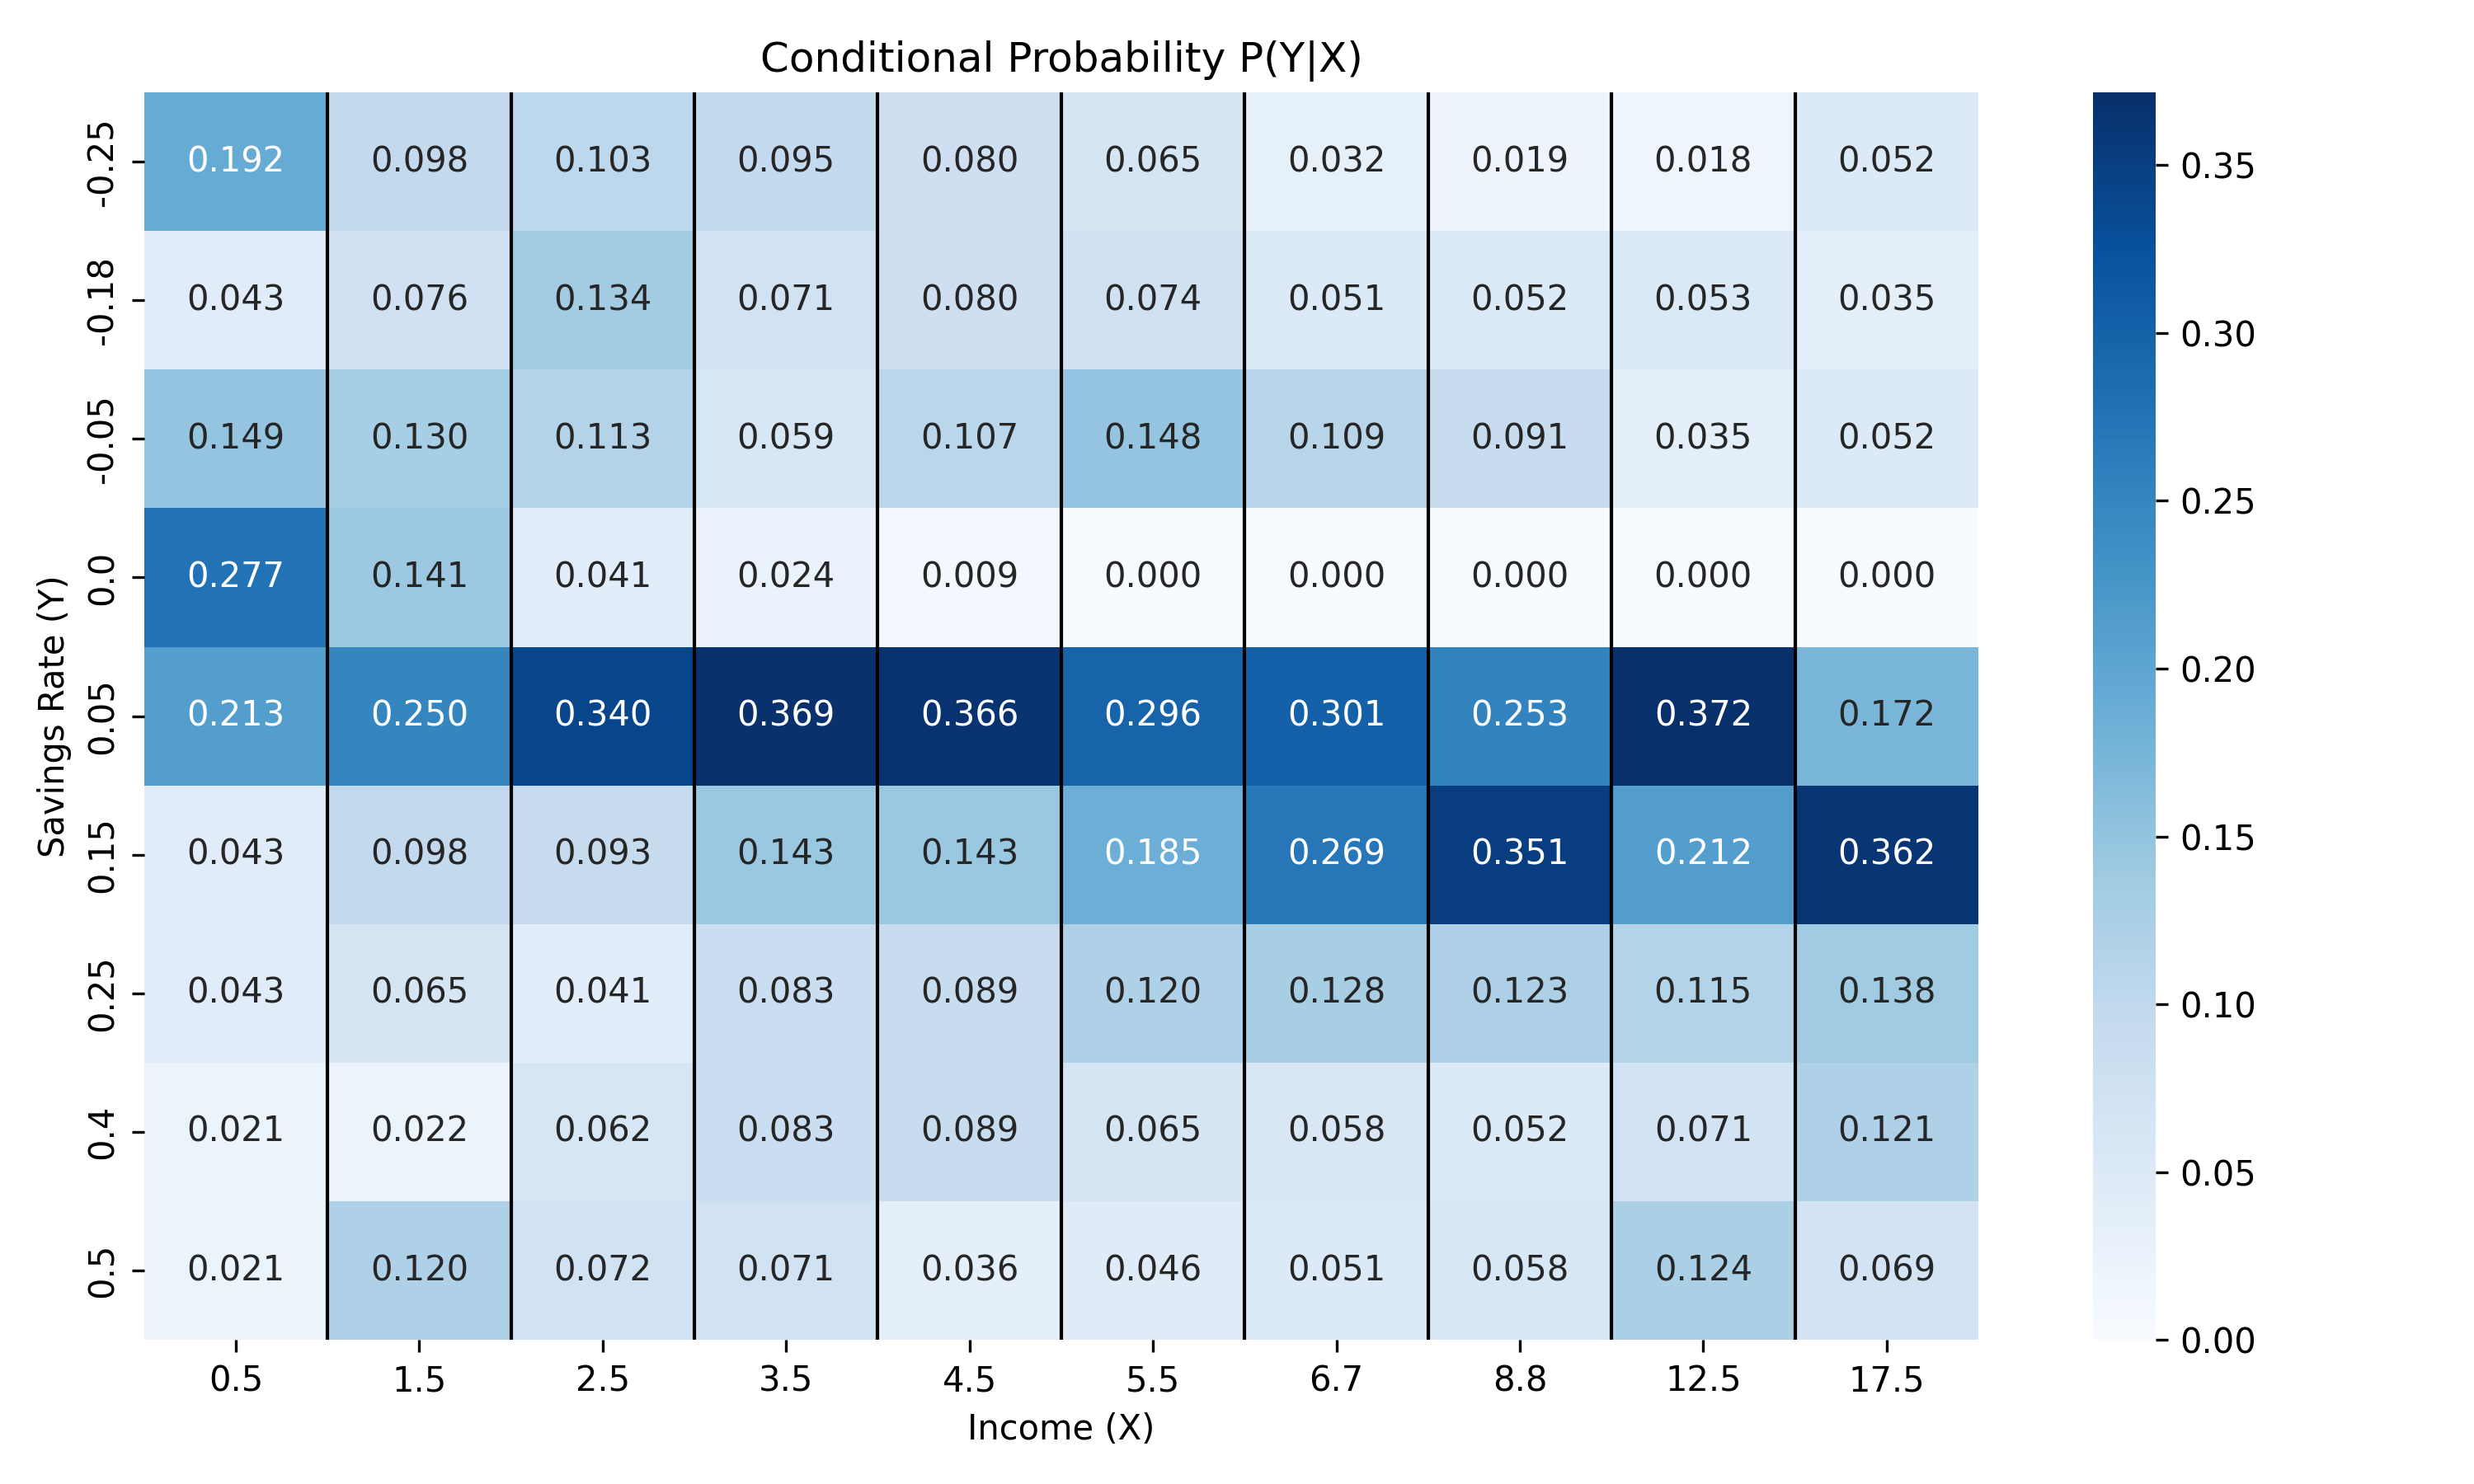
\includegraphics[width=\textwidth]{heatmap_P_Y_given_X.png}
\caption{Conditional probability $P(Y|X)$}
\end{figure}


\subsection*{Interpretation}

Each column of $P_{Y\mid X}$ describes the savings-rate distribution for a given income category. At the lowest income level, 0.5, the probability of zero savings is 0.2766, which is actually larger than the probability of saving 0.15, 0.25, 0.40, or 0.50. In addition, the negative savings categories $-0.25$ and $-0.05$ have probabilities 0.1915 and 0.1489, so dissaving is not unusual among the lowest-income households.

The picture changes as income rises. At income 8.8, the largest probability is attached to a savings rate of 0.15, with value 0.3506, while the probability of zero savings falls to 0. At income 12.5, the most likely savings rate is 0.05 with probability 0.3717, followed by 0.15 with probability 0.2124. At income 17.5, the highest probability is again at 0.15, equal to 0.3621. These patterns suggest that higher-income households are much more likely to appear in positive savings categories and much less likely to report zero or negative savings.




\vspace{\x}
\section*{4. Marginal Means of Income and Savings Rate}

\subsection*{Formula}

The marginal mean of income is
\[
E[X]=\sum_{j=1}^{10}x_j p_X(x_j)=x^\top p_X,
\]
and the marginal mean of savings rate is
\[
E[Y]=\sum_{i=1}^{9}y_i p_Y(y_i)=y^\top p_Y.
\]

\subsection*{Results}

\[
E[X]\approx 6.4877,
\qquad
E[Y]\approx 0.0970.
\]

\subsection*{Interpretation}

The marginal mean of income is 6.4877, which means that the average household income in the sample is about \$6.49 thousand per year. The marginal mean of the savings rate is 0.0970, so the average household saves about 9.7\% of income. These two numbers describe the center of the sample in a simple way: the typical household is neither in the very lowest nor in the very highest income group, and on average it saves a modest positive share of income.




\vspace{\x}
\section*{5. Conditional Mean of Savings Rate Given Income}

\subsection*{Formula}

The conditional mean of savings rate for a given income category $X=x_j$ is
\[
E[Y\mid X=x_j]=\sum_{i=1}^{9} y_i P(Y=y_i\mid X=x_j).
\]

In matrix form,
\[
m_{Y\mid X}=y^\top P_{Y\mid X}.
\]

\subsection*{Results}

\begin{center}
\begin{tabular}{cc}
\toprule
Income & $E[Y\mid X]$ \\
\midrule
0.5  & -0.0162 \\
1.5  & 0.0673 \\
2.5  & 0.0465 \\
3.5  & 0.0901 \\
4.5  & 0.0757 \\
5.5  & 0.0848 \\
6.7  & 0.1135 \\
8.8  & 0.1273 \\
12.5 & 0.1537 \\
17.5 & 0.1584 \\
\bottomrule
\end{tabular}
\end{center}

\subsection*{Interpretation}

The conditional mean of savings generally increases with income, although the pattern is not perfectly monotonic at every point. In the lowest income category, 0.5, the conditional mean is $-0.0162$, which means that households in this group are, on average, slightly dissaving. By contrast, at income 6.7 and 8.8, the conditional means rise to 0.1135 and 0.1273, and they reach 0.1537 and 0.1584 at incomes 12.5 and 17.5.

So, while there are small fluctuations in the middle of the table, the overall pattern is clear: higher-income households tend to save a larger fraction of their income. This is consistent with the conditional distributions reported earlier.




\vspace{\x}
\section*{6. Marginal Variance and Standard Deviation of Income and Savings Rate}

\subsection*{Formula}

The marginal variance of income is
\[
\operatorname{Var}(X)=E[X^2]-\{E[X]\}^2,
\qquad
E[X^2]=\sum_{j=1}^{10}x_j^2 p_X(x_j).
\]

The marginal variance of savings rate is
\[
\operatorname{Var}(Y)=E[Y^2]-\{E[Y]\}^2,
\qquad
E[Y^2]=\sum_{i=1}^{9}y_i^2 p_Y(y_i).
\]

The corresponding standard deviations are
\[
SD(X)=\sqrt{\operatorname{Var}(X)},
\qquad
SD(Y)=\sqrt{\operatorname{Var}(Y)}.
\]

\subsection*{Results}

\[
\operatorname{Var}(X)\approx 18.3768,
\qquad
SD(X)\approx 4.2868.
\]

\[
\operatorname{Var}(Y)\approx 0.0357,
\qquad
SD(Y)\approx 0.1889.
\]

\subsection*{Interpretation}

The variance of income is 18.3768 and the corresponding standard deviation is 4.2868. Since income is measured in thousands of dollars, this means that household incomes are spread quite widely around the mean of 6.4877. In other words, the sample contains substantial income heterogeneity rather than being tightly concentrated around a single middle category.

For savings rates, the variance is 0.0357 and the standard deviation is 0.1889. Relative to the mean savings rate of 0.0970, this is fairly large, which suggests that savings behavior differs considerably across households. Some households save quite a bit, while others save very little or even report negative savings.




\vspace{\x}
\section*{7. Conditional Variance and Standard Deviation of Savings Rate Given Income}

\subsection*{Formula}

For a given income category $X=x_j$, the conditional variance of savings rate is
\[
\operatorname{Var}(Y\mid X=x_j)
=
E[Y^2\mid X=x_j]-\{E[Y\mid X=x_j]\}^2,
\]
where
\[
E[Y^2\mid X=x_j]
=
\sum_{i=1}^{9} y_i^2 P(Y=y_i\mid X=x_j).
\]

In matrix form,
\[
s_{Y\mid X}=(y\odot y)^\top P_{Y\mid X},
\qquad
v_{Y\mid X}=s_{Y\mid X}-m_{Y\mid X}\odot m_{Y\mid X}.
\]

The conditional standard deviation is
\[
SD(Y\mid X=x_j)=\sqrt{\operatorname{Var}(Y\mid X=x_j)}.
\]

\subsection*{Results}

\begin{center}
\begin{tabular}{cccc}
\toprule
Income & $E[Y\mid X]$ & $\operatorname{Var}(Y\mid X)$ & $SD(Y\mid X)$ \\
\midrule
0.5  & -0.0162 & 0.0263 & 0.1623 \\
1.5  & 0.0673  & 0.0447 & 0.2113 \\
2.5  & 0.0465  & 0.0424 & 0.2058 \\
3.5  & 0.0901  & 0.0408 & 0.2021 \\
4.5  & 0.0757  & 0.0351 & 0.1873 \\
5.5  & 0.0848  & 0.0340 & 0.1844 \\
6.7  & 0.1135  & 0.0279 & 0.1671 \\
8.8  & 0.1273  & 0.0261 & 0.1615 \\
12.5 & 0.1537  & 0.0345 & 0.1857 \\
17.5 & 0.1584  & 0.0331 & 0.1820 \\
\bottomrule
\end{tabular}
\end{center}

\subsection*{Interpretation}

The conditional standard deviation of savings is relatively high at the lower income levels. For example, it is 0.2113 at income 1.5 and 0.2058 at income 2.5, which indicates substantial variation in saving behavior within those groups. Even among households with similarly low incomes, some save, some do not save, and some dissave.

As income moves into the middle range, the dispersion becomes smaller. At income 6.7 and 8.8, the conditional standard deviations fall to 0.1671 and 0.1615, respectively, which are the lowest values in the table. At higher income levels such as 12.5 and 17.5, the standard deviations increase slightly again to 0.1857 and 0.1820, but they remain below the earlier peak. This suggests that saving behavior becomes more stable in the middle-to-higher income range, although some heterogeneity is still present.




\vspace{\x}
\section*{Conclusion}

Overall, the results point to a positive relationship between income and savings. The marginal distributions show that most households are concentrated in the middle and upper-middle income categories and in small positive savings categories, especially 0.05 and 0.15. The conditional distributions reinforce this pattern: lower-income households are more likely to have zero or negative savings, while higher-income households are more likely to appear in the positive savings categories.

The summary statistics tell a similar story. The average income is 6.4877 and the average savings rate is 0.0970, while the conditional mean of savings rises from $-0.0162$ at income 0.5 to 0.1584 at income 17.5. In addition, the conditional standard deviations suggest that saving behavior is more dispersed among lower-income households and somewhat more stable in the middle-income range. Taken together, the evidence consistently suggests that households with higher income tend to save more.

\vspace{20em}
\noindent
\textit{This report was prepared with the assistance of AI tools for translation, mathematical formatting, and Python-based data processing and visualization. All interpretations and conclusions are the author’s own.}



\appendix
\section*{Appendix: Python Code}

\begin{lstlisting}
import numpy as np
import pandas as pd

# =========================================================
# [기본 데이터 설정]
# =========================================================

# Income categories
# 단위: $1000/year
# 예: 0.5 는 연소득 500달러, 17.5 는 연소득 17,500달러를 의미
x = np.array([0.5, 1.5, 2.5, 3.5, 4.5, 5.5, 6.7, 8.8, 12.5, 17.5])

# Savings rate categories
# 단위: 비율 자체
# 예: 0.05 = 5%, -0.25 = -25%
y = np.array([-0.25, -0.18, -0.05, 0.00, 0.05, 0.15, 0.25, 0.40, 0.50])

# Frequency matrix N
# 행(row) = savings rate category
# 열(col) = income category
# 각 원소 n_ij = (저축률 i, 소득 j)에 속하는 가구 수
N = np.array([
    [ 9,  9, 10,  8,  9,  7,  5,  3,  2,  3],
    [ 2,  7, 13,  6,  9,  8,  8,  8,  6,  2],
    [ 7, 12, 11,  5, 12, 16, 17, 14,  4,  3],
    [13, 13,  4,  2,  1,  0,  0,  0,  0,  0],
    [10, 23, 33, 31, 41, 32, 47, 39, 42, 10],
    [ 2,  9,  9, 12, 16, 20, 42, 54, 24, 21],
    [ 2,  6,  4,  7, 10, 13, 20, 19, 13,  8],
    [ 1,  2,  6,  7, 10,  7,  9,  8,  8,  7],
    [ 1, 11,  7,  6,  4,  5,  8,  9, 14,  4]
])

# 전체 표본수 n
# 문제에서 총 1021가구라고 했고, 실제로 합이 1021인지 확인
n = N.sum()
print("Total sample size n =", n)

# Joint probability matrix P
# 각 셀의 도수를 전체 표본수 n으로 나눈 값
# 즉, p_ij = n_ij / n
P = N / n

# 보기 좋게 표 형태로 확인하기 위한 라벨
income_labels = [f"{v:g}" for v in x]
savings_labels = [f"{v:g}" for v in y]

# 도수표 DataFrame
freq_df = pd.DataFrame(
    N,
    index=savings_labels,
    columns=income_labels
)

# 결합확률표 DataFrame
prob_df = pd.DataFrame(
    P,
    index=savings_labels,
    columns=income_labels
)

print("\nFrequency table N:")
print(freq_df)

print("\nJoint probability table P = N/n:")
print(prob_df.round(4))


# =========================================================
# [자주 쓰는 기본 합]
# =========================================================

# income의 주변도수 = 열합
# 각 income category에 속한 전체 가구 수
col_freq = N.sum(axis=0)

# savings rate의 주변도수 = 행합
# 각 savings category에 속한 전체 가구 수
row_freq = N.sum(axis=1)

# income의 주변확률 = 열합 / n
col_prob = P.sum(axis=0)

# savings의 주변확률 = 행합 / n
row_prob = P.sum(axis=1)


# =========================================================
# 1번: Marginal frequencies of income and savings rate
# =========================================================

# Income marginal frequencies
# 열 기준 합 -> 각 소득범주의 전체 빈도
income_marg_freq = N.sum(axis=0)

# Savings marginal frequencies
# 행 기준 합 -> 각 저축률범주의 전체 빈도
savings_marg_freq = N.sum(axis=1)

# 주변확률 = 주변도수 / 전체표본수
income_marg_prob = income_marg_freq / n
savings_marg_prob = savings_marg_freq / n

print("\n[1] Income marginal frequencies:")
print(income_marg_freq)

print("\n[1] Income marginal probabilities:")
print(np.round(income_marg_prob, 4))

print("\n[1] Savings marginal frequencies:")
print(savings_marg_freq)

print("\n[1] Savings marginal probabilities:")
print(np.round(savings_marg_prob, 4))


# =========================================================
# 2번: Conditional frequencies of income, conditional on savings
# =========================================================

# P(X | Y)
# 특정 savings rate가 주어졌을 때 income 분포
# 각 행을 그 행의 합(row total)으로 나눔
# 즉, P(X=x_j | Y=y_i) = n_ij / sum_j n_ij
row_freq = N.sum(axis=1)
cond_income_given_savings = N / row_freq[:, None]

cond_df = pd.DataFrame(
    cond_income_given_savings,
    index=savings_labels,
    columns=income_labels
)

print("\n[2] Conditional probabilities of income given savings, P(X|Y):")
print(cond_df.round(4))


# =========================================================
# 3번: Conditional frequencies of savings rate, conditional on income
# =========================================================

# P(Y | X)
# 특정 income이 주어졌을 때 savings rate 분포
# 각 열을 그 열의 합(column total)으로 나눔
# 즉, P(Y=y_i | X=x_j) = n_ij / sum_i n_ij
col_freq = N.sum(axis=0)
cond_savings_given_income = N / col_freq[None, :]

cond_df2 = pd.DataFrame(
    cond_savings_given_income,
    index=savings_labels,
    columns=income_labels
)

print("\n[3] Conditional probabilities of savings given income, P(Y|X):")
print(cond_df2.round(4))


# =========================================================
# 4번: Marginal mean of income and savings rate
# =========================================================

# income의 주변확률벡터 p_X
income_marg_prob = P.sum(axis=0)

# savings의 주변확률벡터 p_Y
savings_marg_prob = P.sum(axis=1)

# E[X] = sum(x_j * p_Xj)
mu_X = x @ income_marg_prob

# E[Y] = sum(y_i * p_Yi)
mu_Y = y @ savings_marg_prob

print("\n[4] Marginal mean of income =", round(mu_X, 4))
print("[4] Marginal mean of savings rate =", round(mu_Y, 4))


# =========================================================
# 5번: Conditional mean of savings rate, conditional on income
# =========================================================

# 이미 구한 P(Y|X)를 다시 사용
col_freq = N.sum(axis=0)
cond_savings_given_income = N / col_freq[None, :]

# 각 income category별 평균 savings rate
# E[Y|X=x_j] = sum(y_i * P(Y=y_i | X=x_j))
cond_mean_savings_given_income = y @ cond_savings_given_income

cond_mean_df = pd.DataFrame({
    "Income": x,
    "E[Savings rate | Income]": cond_mean_savings_given_income
})

print("\n[5] Conditional mean of savings rate given income:")
print(cond_mean_df.round(4))


# =========================================================
# 6번: Marginal variance and standard deviation
# =========================================================

# 주변확률
income_marg_prob = P.sum(axis=0)
savings_marg_prob = P.sum(axis=1)

# 주변평균
mu_X = x @ income_marg_prob
mu_Y = y @ savings_marg_prob

# 제2모멘트
# E[X^2], E[Y^2]
EX2 = (x**2) @ income_marg_prob
EY2 = (y**2) @ savings_marg_prob

# 분산 공식
# Var(X) = E[X^2] - (E[X])^2
# Var(Y) = E[Y^2] - (E[Y])^2
var_X = EX2 - mu_X**2
var_Y = EY2 - mu_Y**2

# 표준편차 = 분산의 제곱근
sd_X = np.sqrt(var_X)
sd_Y = np.sqrt(var_Y)

print("\n[6] Income variance =", round(var_X, 4))
print("[6] Income standard deviation =", round(sd_X, 4))
print("[6] Savings variance =", round(var_Y, 4))
print("[6] Savings standard deviation =", round(sd_Y, 4))


# =========================================================
# 7번: Conditional variance and standard deviation of savings, given income
# =========================================================

# 조건부확률 P(Y|X)
col_freq = N.sum(axis=0)
cond_savings_given_income = N / col_freq[None, :]

# 조건부평균
# E[Y|X=x_j]
cond_mean = y @ cond_savings_given_income

# 조건부 제2모멘트
# E[Y^2 | X=x_j]
cond_second_moment = (y**2) @ cond_savings_given_income

# 조건부분산
# Var(Y|X=x_j) = E[Y^2|X=x_j] - (E[Y|X=x_j])^2
cond_var = cond_second_moment - cond_mean**2

# 조건부표준편차
cond_sd = np.sqrt(cond_var)

cond_var_df = pd.DataFrame({
    "Income": x,
    "E[Y|X]": cond_mean,
    "Var(Y|X)": cond_var,
    "SD(Y|X)": cond_sd
})

print("\n[7] Conditional mean, variance, and standard deviation of savings given income:")
print(cond_var_df.round(4))
\end{lstlisting}

\end{document}